\documentclass{standalone}

   \usepackage[scaled]{helvet}
   \renewcommand\familydefault{\sfdefault}
   \usepackage[T1]{fontenc}
   \usepackage{graphicx}
   \usepackage{pgfplots}

   \pgfplotsset{compat=1.13}
   \definecolor{myblue}{RGB}{81,115,213}

\begin{document}
\begin{tikzpicture}[
      font=\sffamily,
      arrow/.style={->,myblue,line width=.2cm},
      box/.style={myblue,rounded corners=.2cm,line width=.2cm}
   ]
   % Wav File
   \node[inner sep=0pt] at (-0.75,-0.05) {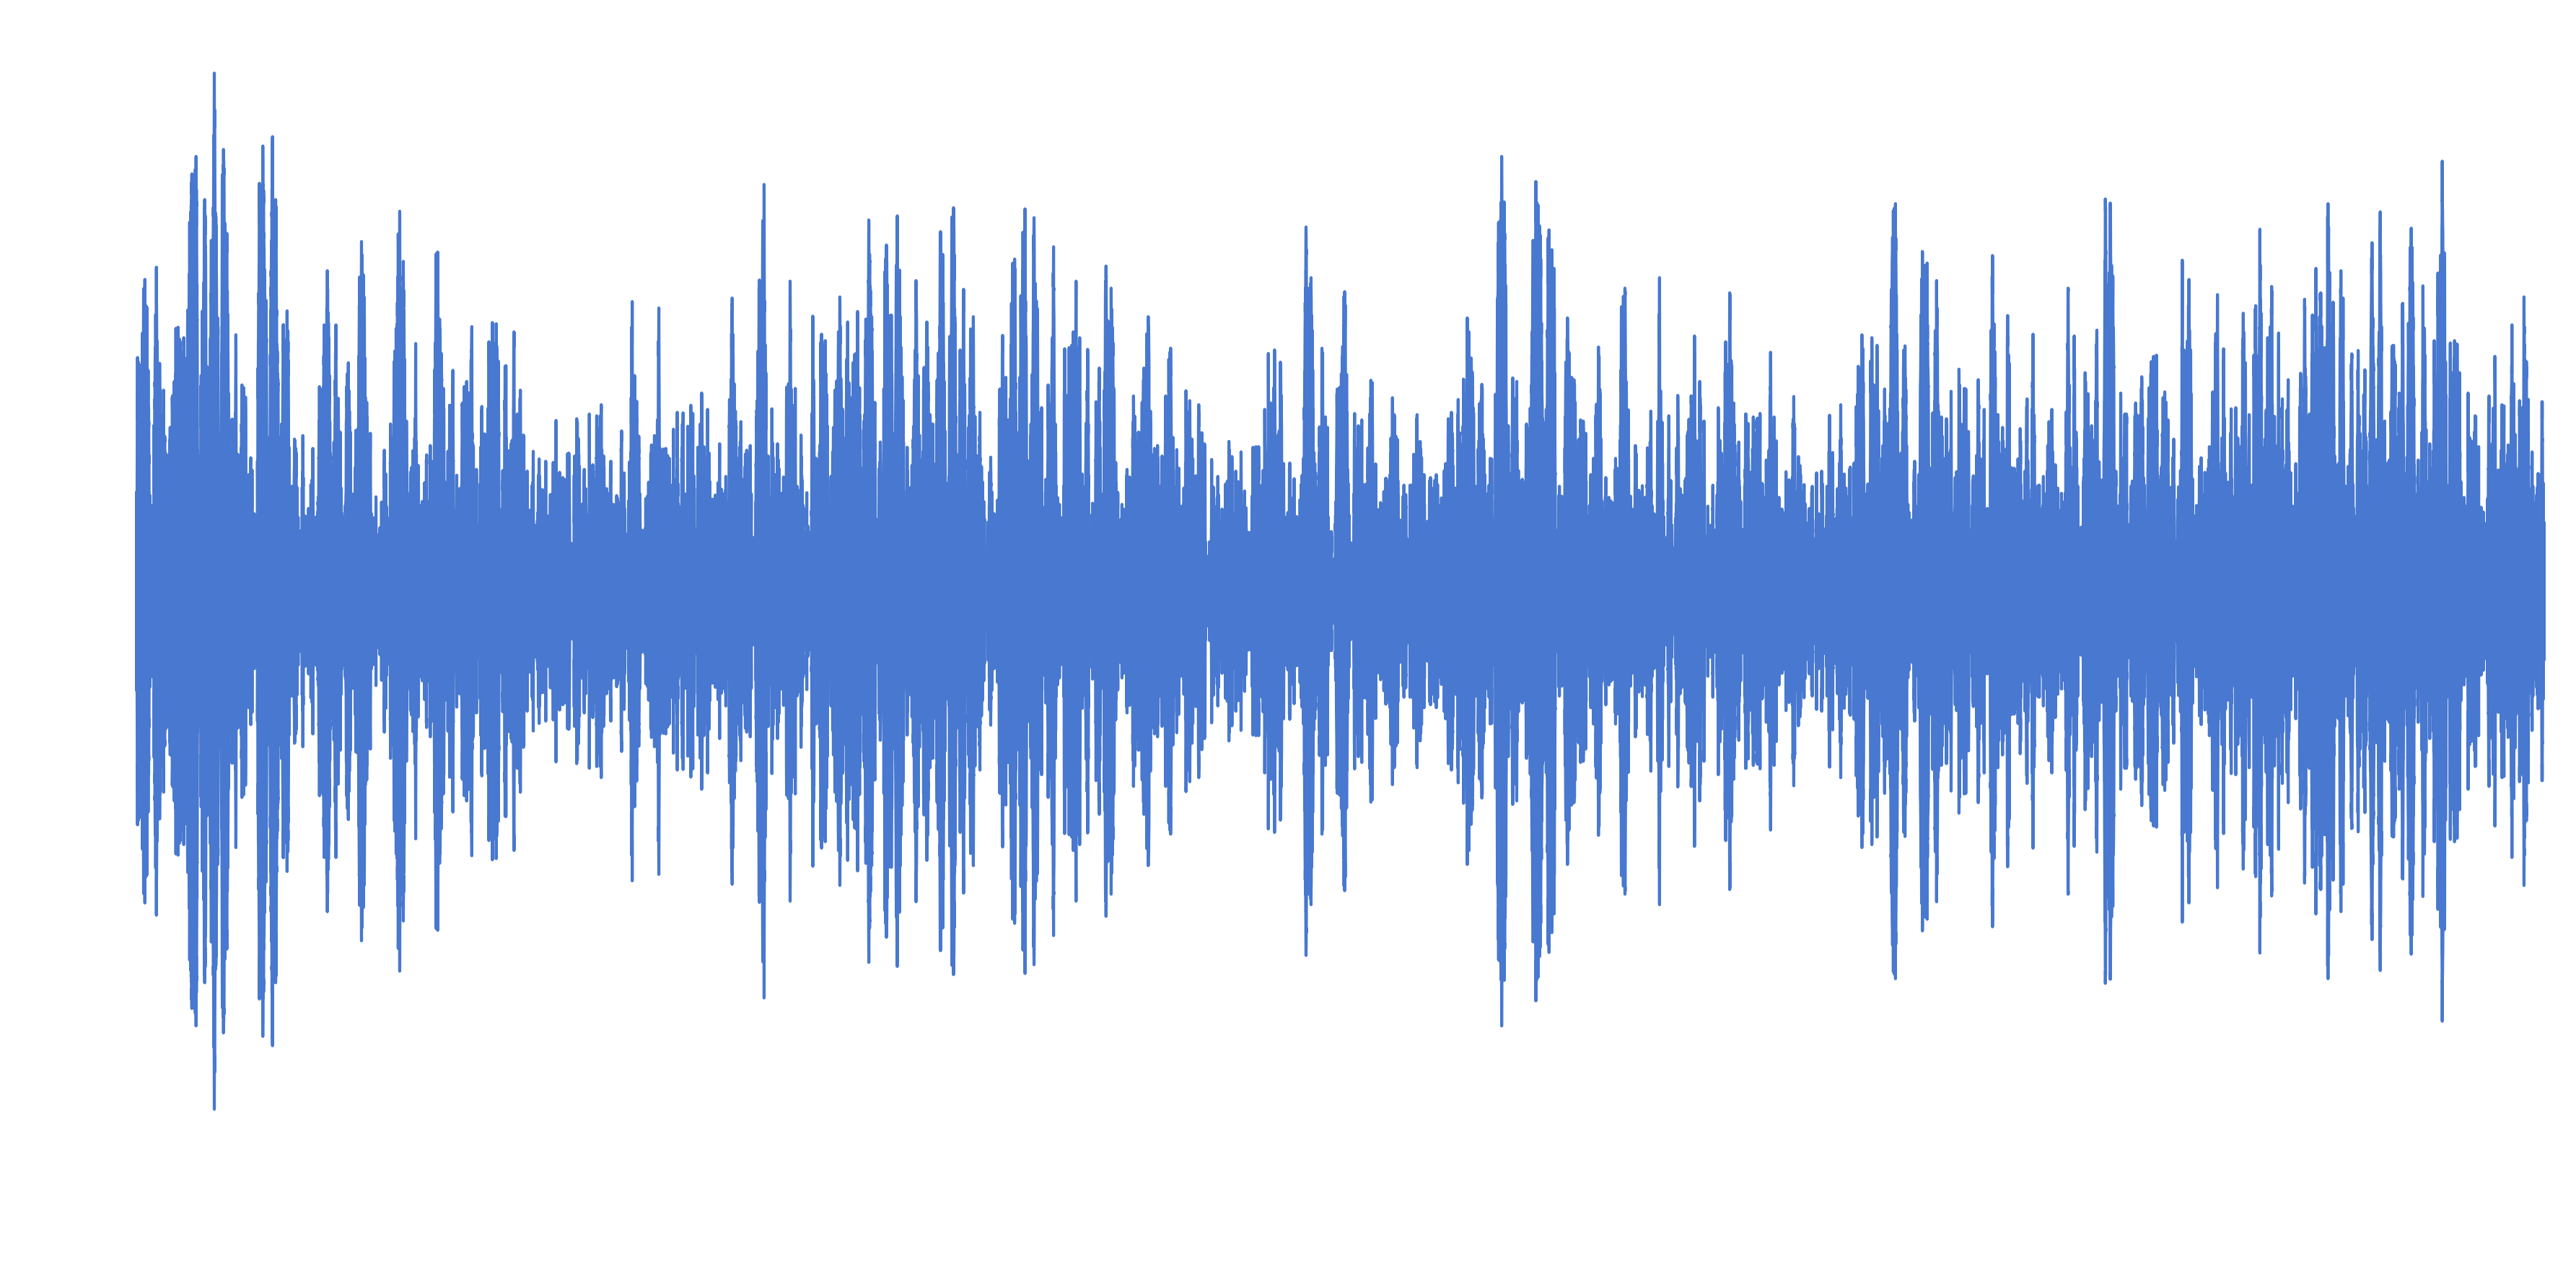
\includegraphics[width=3cm]{images/waveform}};
   \draw[arrow, line width=1.5pt] (1,0) -- (1.75,0) node{};

   % Box around STFT equation
   \pgfmathsetmacro{\cubex}{2.75};
   \pgfmathsetmacro{\cubey}{1};
   \draw[box, line width=1.5pt] (4.75,0.5,0) -- ++(-\cubex,0,0) -- ++(0,-\cubey,0) -- ++(\cubex,0,0) -- cycle;
   \node[text width=3cm] (fft) at (4.25,0) {\Large STFT};
   \draw[arrow, line width=1.5pt] (5,0) -- (5.75,0) node{};

   % Box around interpolation equation
   \pgfmathsetmacro{\cubex}{4.25};
   \pgfmathsetmacro{\cubey}{1};
   \draw[box, line width=1.5pt] (10.25,0.5,0) -- ++(-\cubex,0,0) -- ++(0,-\cubey,0) -- ++(\cubex,0,0) -- cycle;
   \node[text width=4cm] (fft) at (8.8,0) {\Large Interpolation};
   \draw[arrow, line width=1.5pt] (10.5,0.15) -- (11.25,0.45) node{};
   \draw[arrow, line width=1.5pt] (10.5,0) -- (11.25,0) node{};
   \draw[arrow, line width=1.5pt] (10.5,-0.15) -- (11.25,-0.45) node{};

   % Interpolated spectrograms
   \node[inner sep=0pt] at (12,0.15) {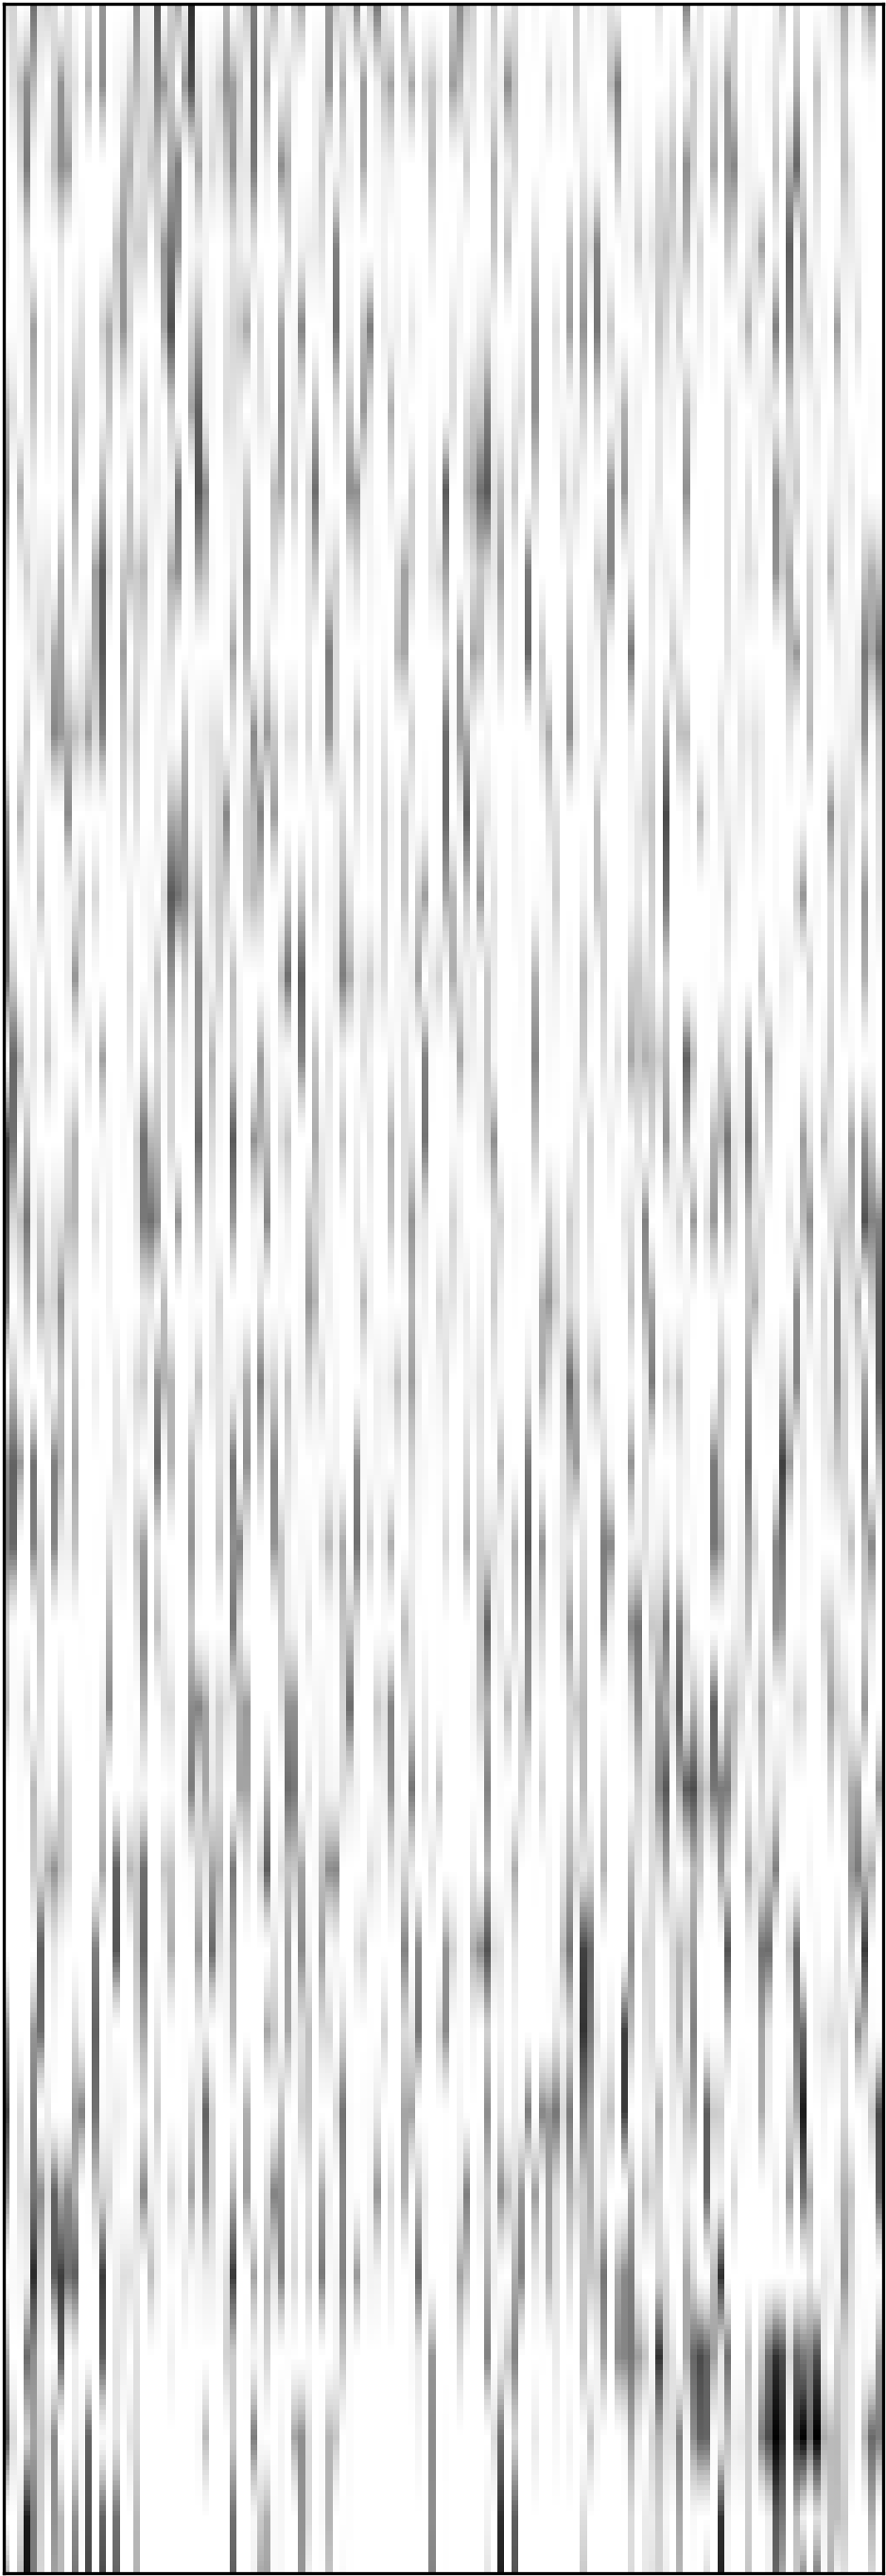
\includegraphics[width=1cm]{images/F_nfft_256}};
   \node[inner sep=0pt] at (12.25,0.00) {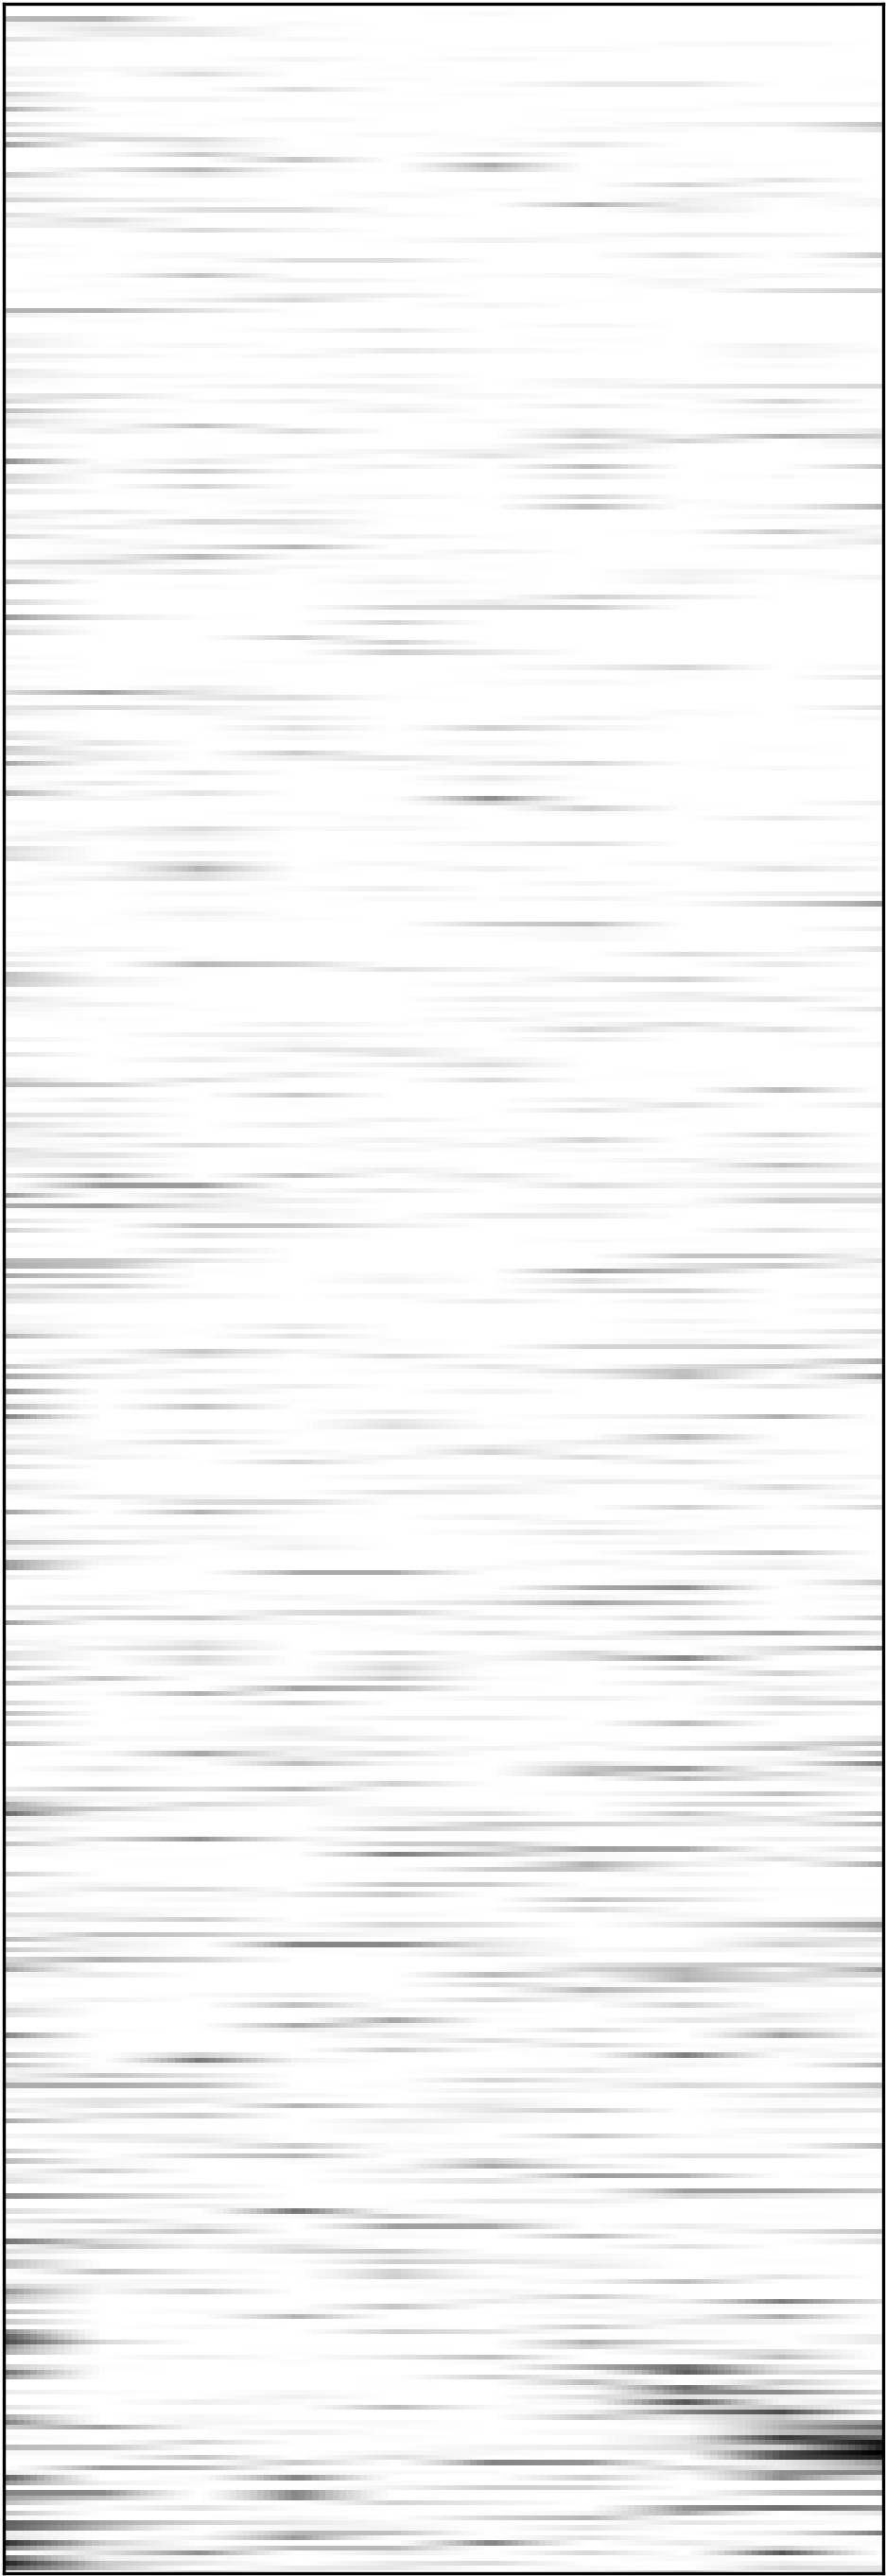
\includegraphics[width=1cm]{images/F_nfft_16384}};
   \node[inner sep=0pt] at (12.5,-0.15) {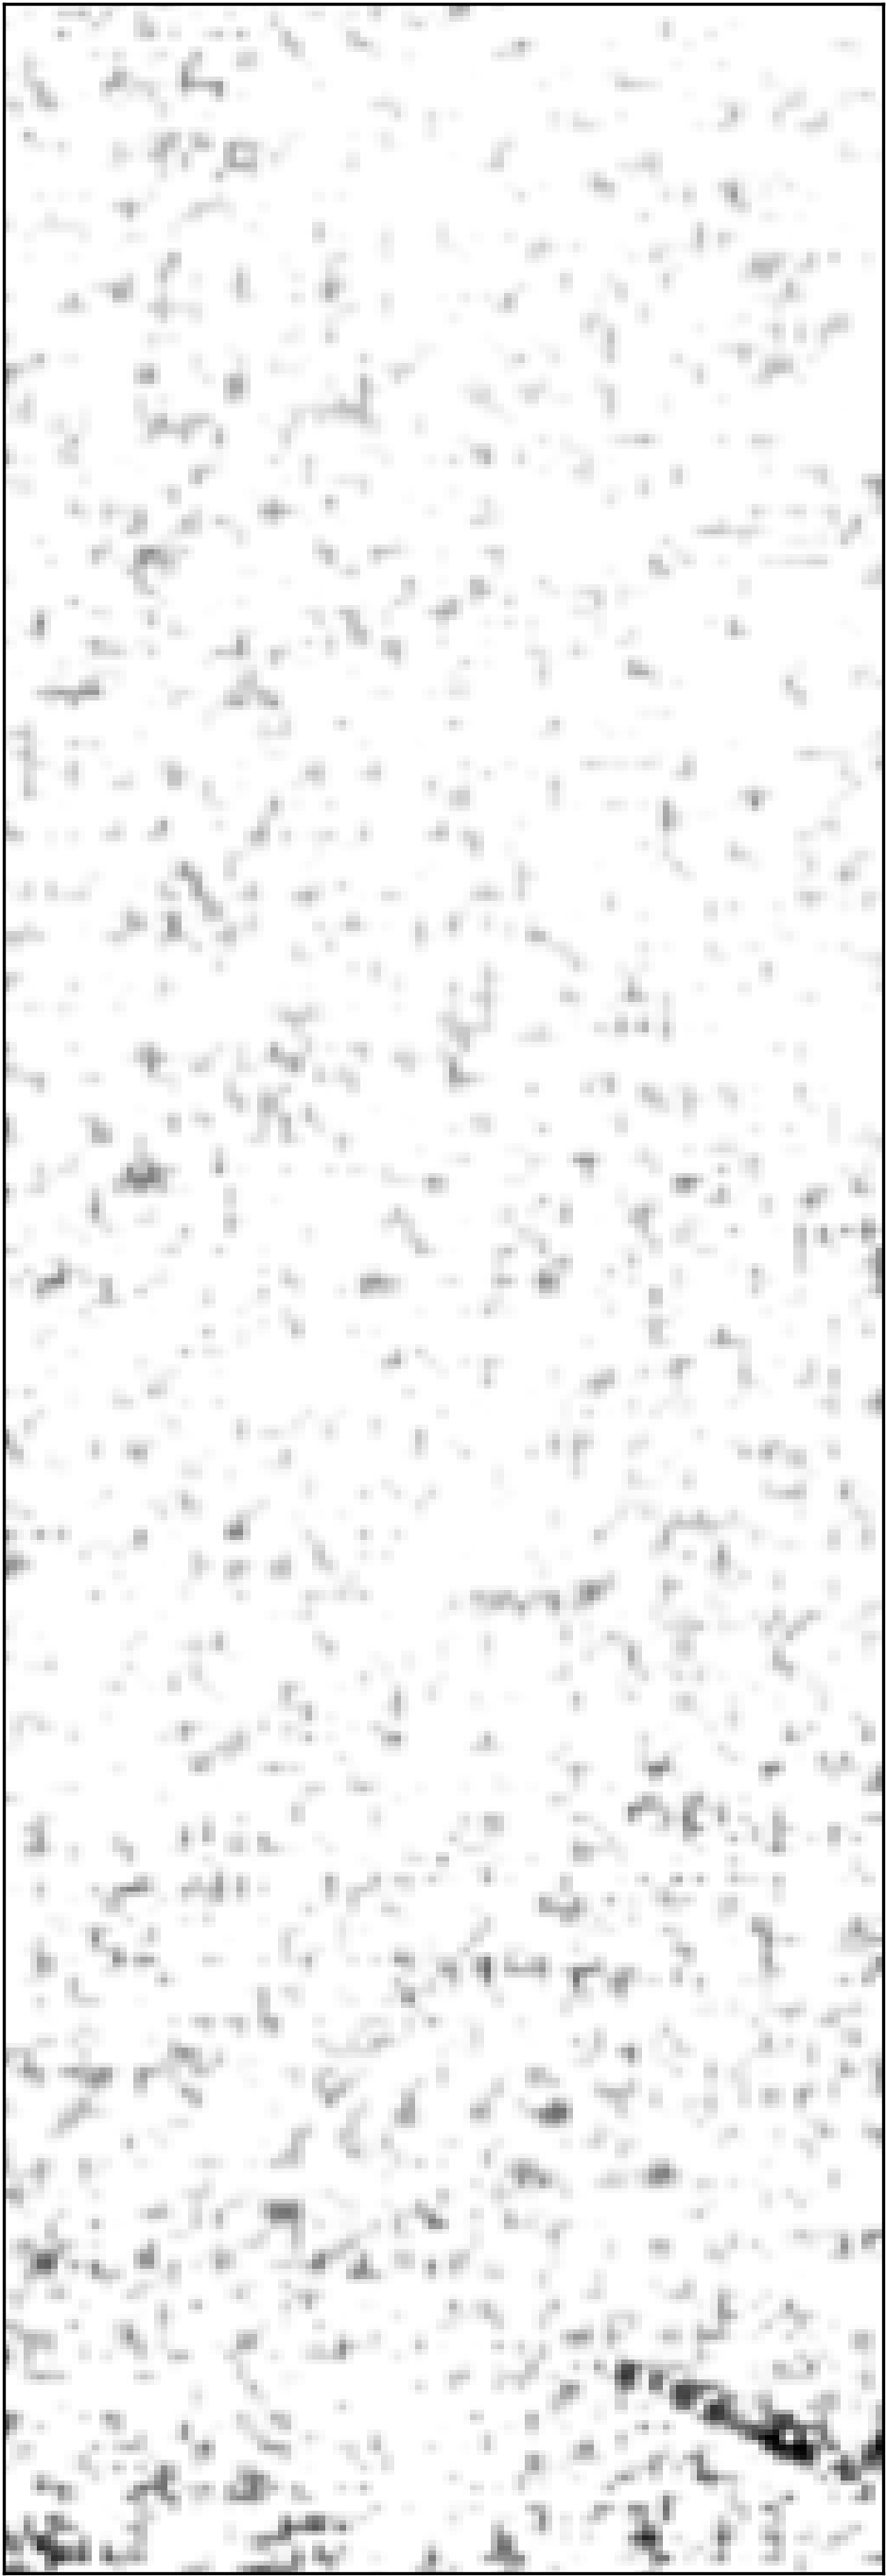
\includegraphics[width=1cm]{images/F_nfft_2048}};
\end{tikzpicture}
\end{document}
